\section{Introduction}

Magnetic Resonance Imaging (MRI) provides an excellent modality for distinguishing different tissues in the
human body, which is essential for medical applications. When MRI is used for stereotactic treatment planning,
its geometric accuracy is crucial. Previous studies have been conducted to correct the distortion caused by
nonlinearity of the MRI scanner’s magnetic gradient fields by imaging a cubic phantom \cite{simple_approach},
\cite{tlee_iaeng} and defining
distortion correction functions based on the distorted appearance its surfaces. Correct mathematical handling
of the distortion correction function required that the cube was centered about the magnetic isocenter, which
is defined as the common center of the three magnetic gradient fields and  is not very accurately known.
New 3-Tesla MRI systems have a larger bore, making the previous phantom design impractically small for probing
the field nonlinearity in the periphery of the bore, as the phantom cannot be scaled up due to constraints
related to weight and cost of manufacturing. We are introducing a new phantom design using a different
approach, which can be built to a larger size, improves accuracy of distortion characterization, and reduces
cost.

\section{Initial Design}

The original phantom design, a 16-cm oil-filled cube, could not be scaled up due to weight and manufacturing
constraints. Our first modification was to look at changing the material to FR-4 since it is rigid, very flat,
and could be submerged for short periods of time to permit scanning the solid liquid interface in an MRI
machine.  Since most of the distortion is visible only in the corners, this was rapidly replaced by 8 corners
of a virtual cube, which could be connected by a rigid frame.  The weight of a tank to submerge either of
these designs to allow scanning was prohibitive, requiring a complete redesign.

\begin{figure}[htb]
  \begin{minipage}[b]{2.75in}
    \centering
    \centerline{\mbox{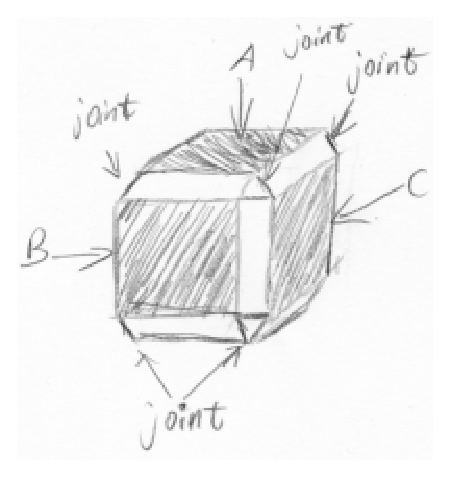
\includegraphics[width=2.75in]{phantom/images/brain_storm/model1.eps}}}
    \centerline{\emph{(a) First model}}
  \end{minipage}\medskip
  \begin{minipage}[b]{2.75in}
    \centering
    \centerline{\mbox{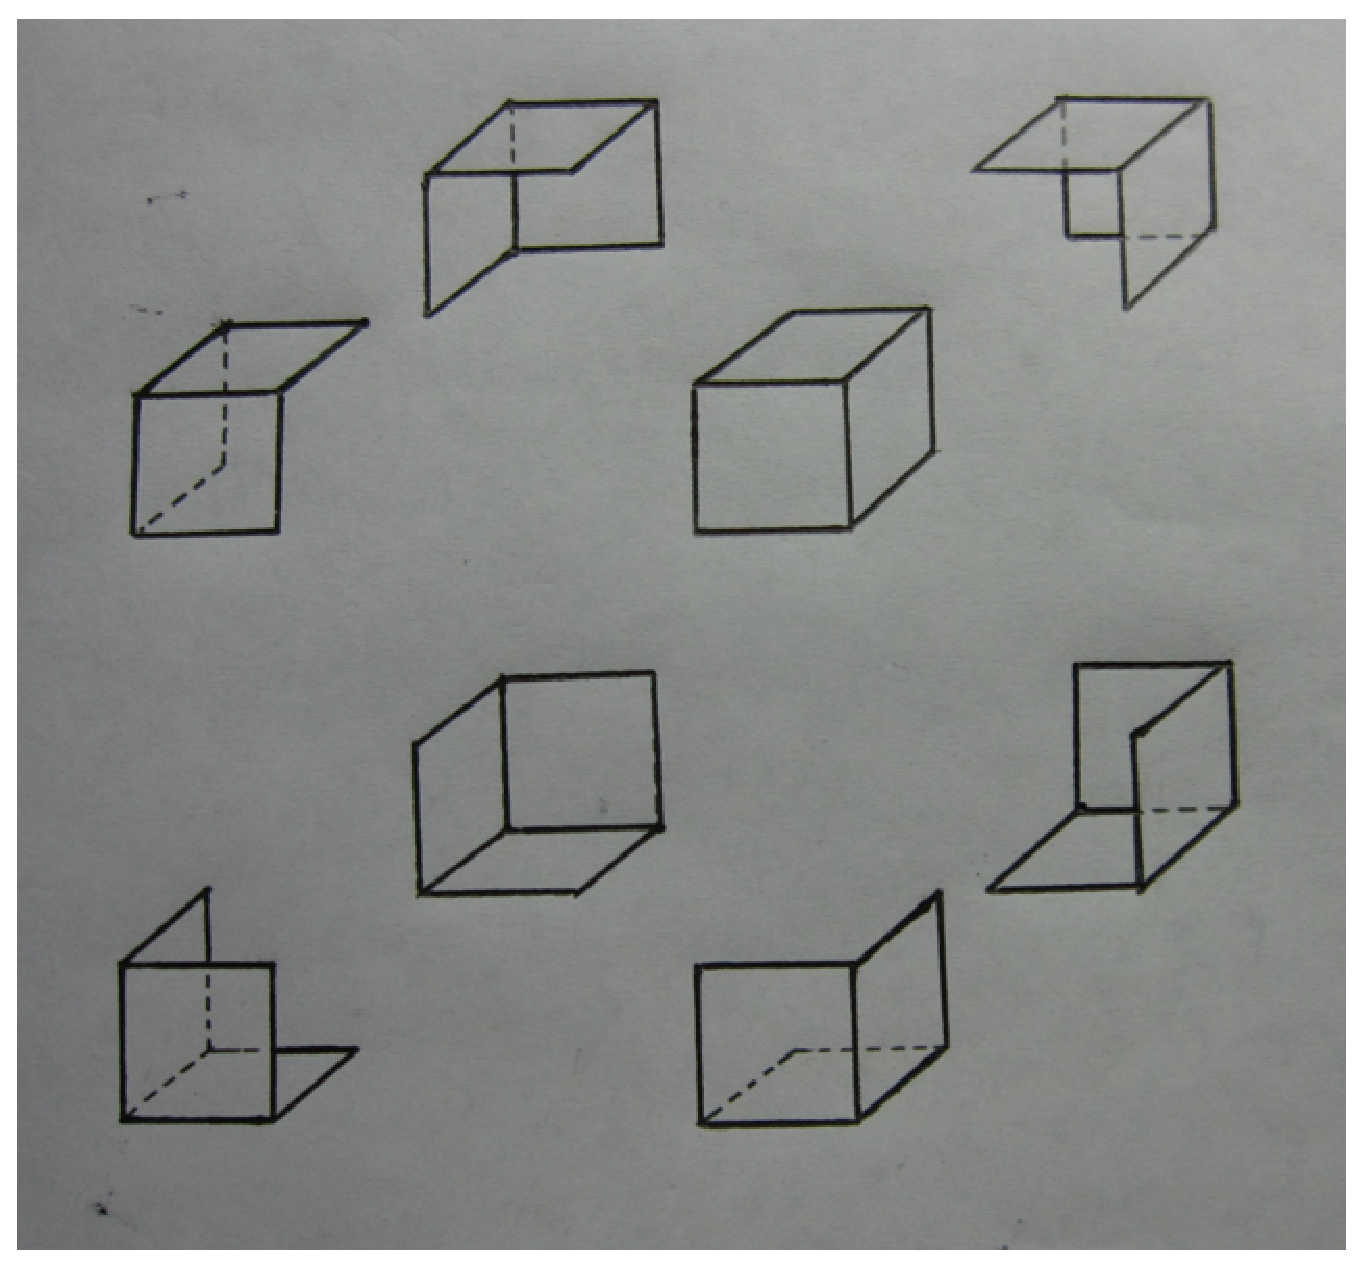
\includegraphics[width=2.75in]{phantom/images/brain_storm/model2.eps}}}
    \centerline{\emph{(b) Second model}}
  \end{minipage}
\end{figure}


\section{New Design}

The phantom is shaped to be as large as possible, while still fitting in the head coil of the scanner, so as
to achieve the maximum quality of signal and largest distortion. The phantom is an octagonal prism with 205 mm
between opposite sides.  Each face of the octagonal prism is composed of 8 high precision NMR tubes that are
5mm in outer diameter and 205 mm in length. These tubes are filled with copper sulfate solution to generate a
strong signal in an MRI scanner.  The tubes are placed parallel to the magnetic field so they will cause less
susceptibility distortion \cite{mag_susceptibility},
and thus provide more accurate information on the gradient field.  In the
center of the phantom is a large water tank to help intensify the signals generated by the tubes. At one end
of the phantom is a cylindrical tank filled with copper sulfate, with a number of small solid cylinders in a
hexagonal pattern that are connecting the two surfaces of the tank. These cylinders are used to maintain the
long-term accuracy of the two surfaces, making sure they won’t deform, and are also aligned to the field to
minimize their effect on the field.  The data generated from 64 tubes mounted on the sides are designed to
give us x and y axis distortion information, and the end tank is designed to provide z-axis distortion data,
allowing a complete 3-D distortion correction with a relatively small amount of data.

\section{Sealing NMR Tubes}

Our original idea for sealing the NMR tubes was to use paraffin wax, either with or without a silicon seal.
Paraffin was heated and a liquid drop was then added to the tube as a seal , but had an uneven bottom caused
by the rapid solidifying of the wax, when it came in contact with the copper sulfate.  Additionally,
it tended to trap air bubbles, which made the end very hard to work with in the images.  Worst yet, after a
few weeks the liquid level in the tubes started to drop.  We decided to compare three potential alternatives:
machinable wax, water weld, and silicon sealer.  As the images on the right show, the silicon was far and
away the best.  There was no leakage lost, and since the setup time was slower on the liquid side it ended
up being almost completely flat.  Every feature was met, and it was also the most cost effective solution.

\begin{figure}[htb]
  \begin{minipage}[b]{1in}
    \centering
    \centerline{\mbox{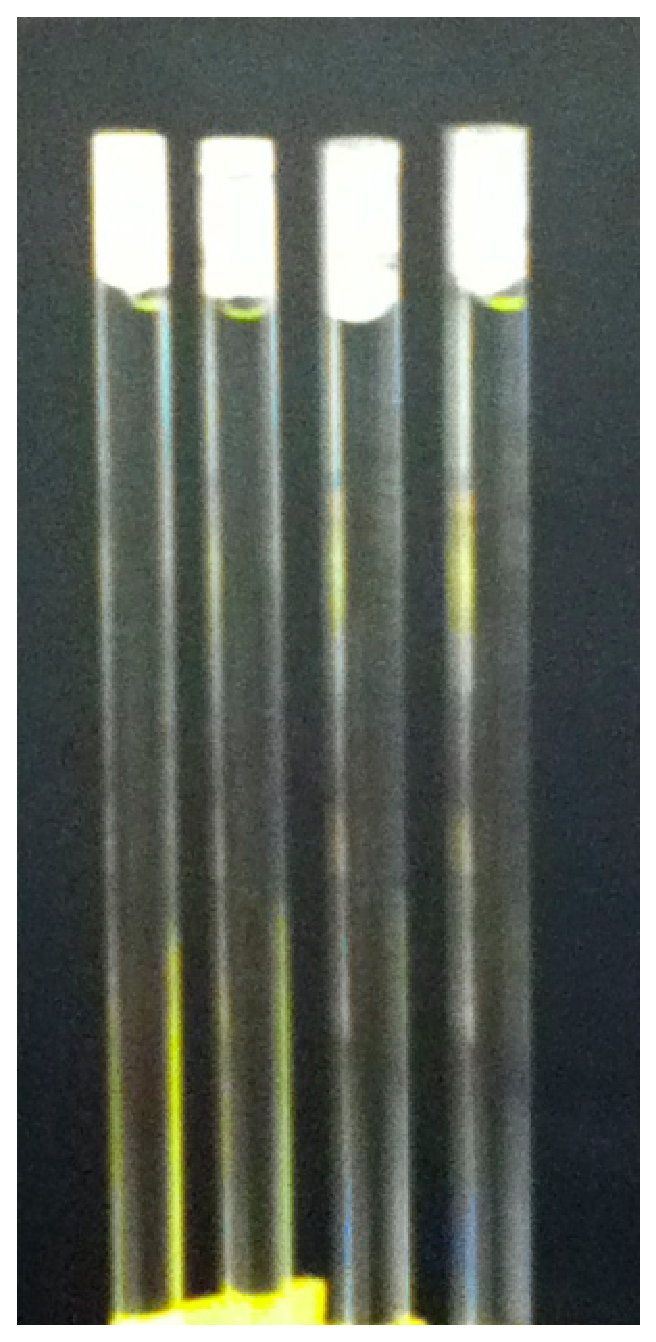
\includegraphics[width=1in]{phantom/images/tube_sealings/paraffin_and_floable_silicon.eps}}}
    \centerline{\emph{(a)}}
  \end{minipage}
  \begin{minipage}[b]{1in}
    \centering
    \centerline{\mbox{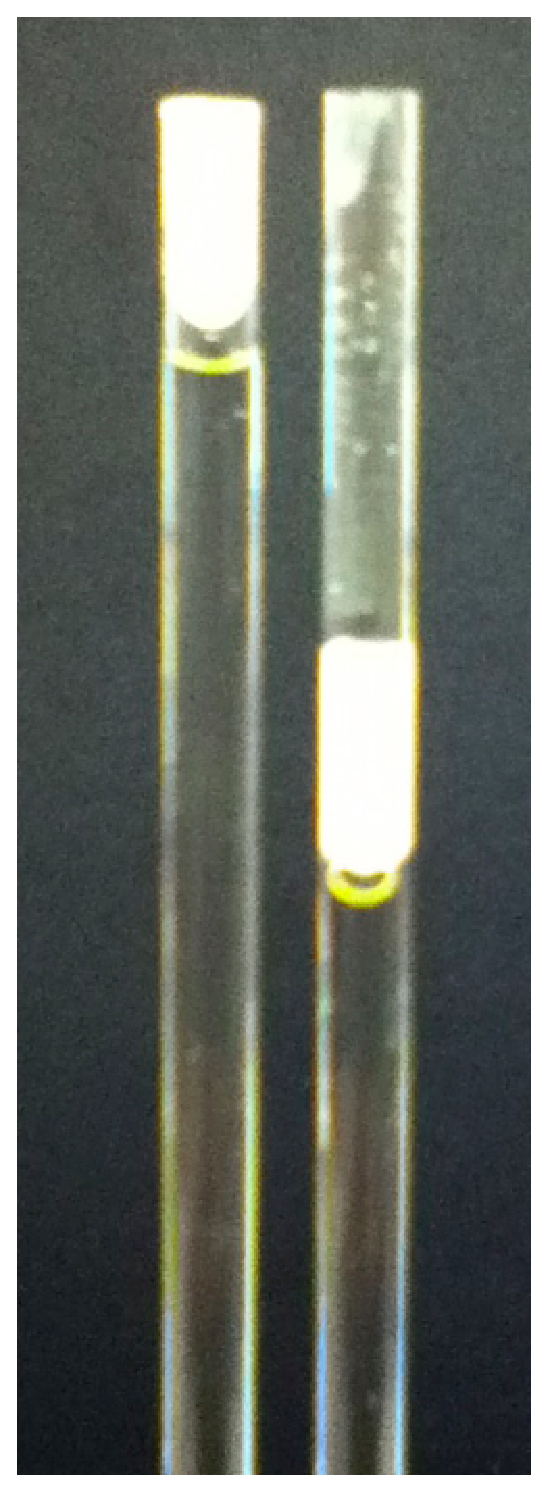
\includegraphics[width=1in]{phantom/images/tube_sealings/paraffin.eps}}}
    \centerline{\emph{(b)}}
  \end{minipage}
  \begin{minipage}[b]{1in}
    \centering
    \centerline{\mbox{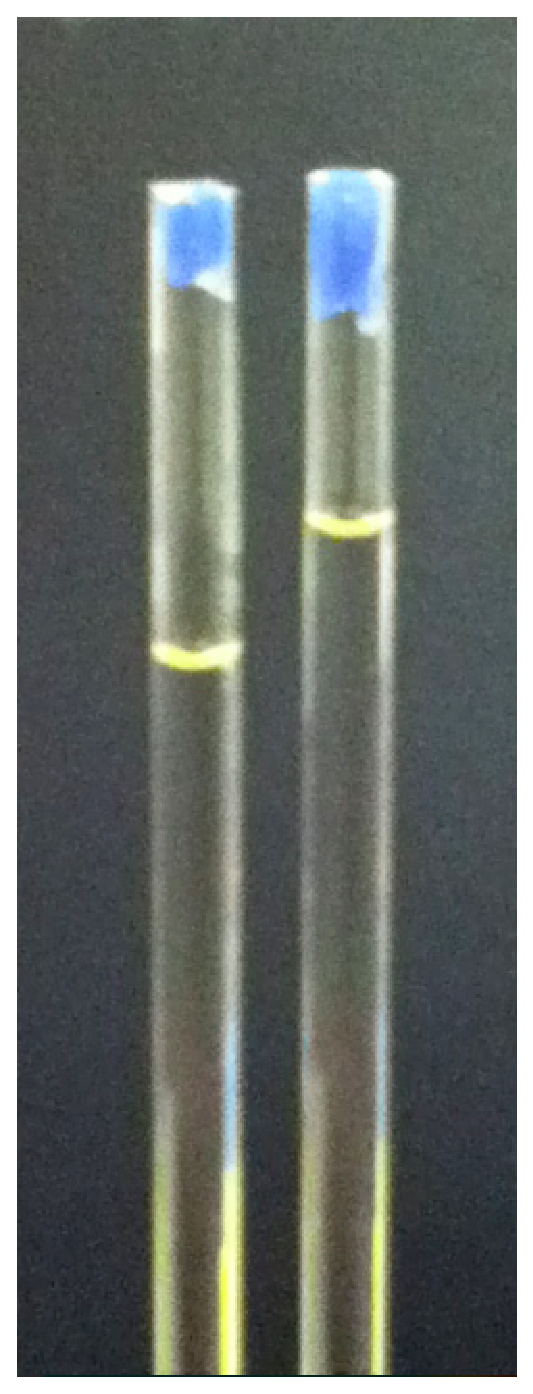
\includegraphics[width=1in]{phantom/images/tube_sealings/machinable_wax.eps}}}
    \centerline{\emph{(c)}}
  \end{minipage}
  \begin{minipage}[b]{1in}
    \centering
    \centerline{\mbox{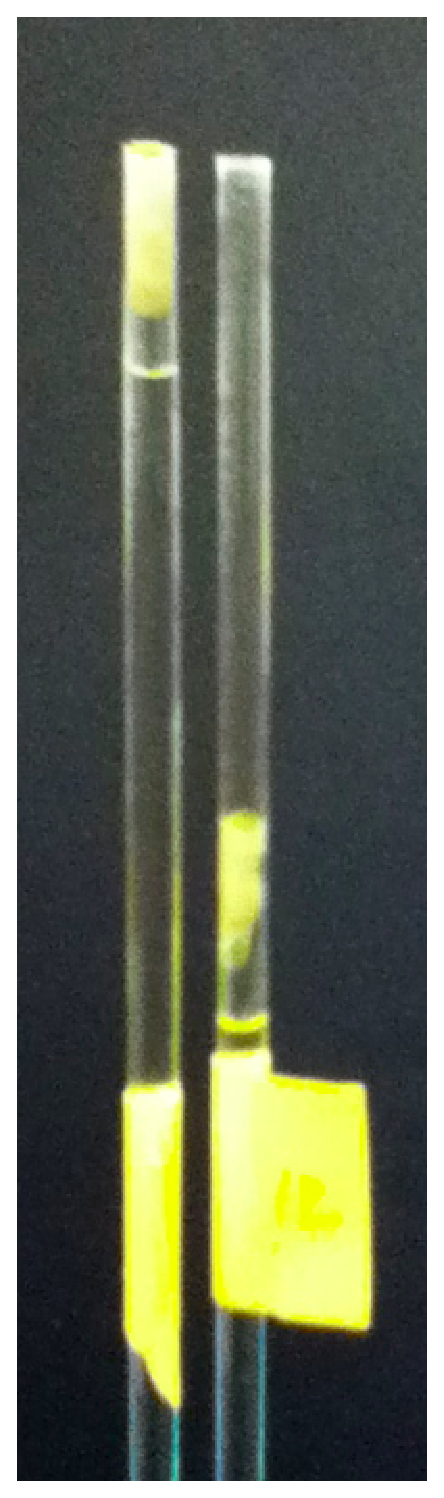
\includegraphics[width=1in]{phantom/images/tube_sealings/water_weld.eps}}}
    \centerline{\emph{(d)}}
  \end{minipage}
  \begin{minipage}[b]{1in}
    \centering
    \centerline{\mbox{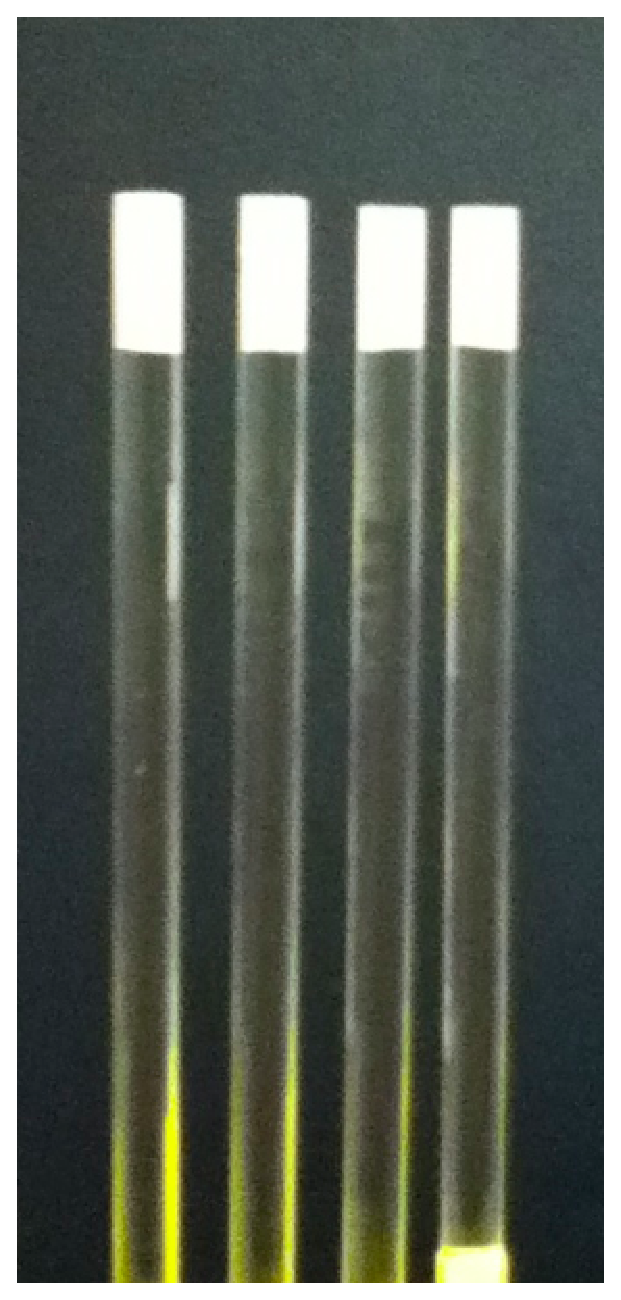
\includegraphics[width=1in]{phantom/images/tube_sealings/silicon.eps}}}
    \centerline{\emph{(e)}}
  \end{minipage}
  \caption{\emph{(a) Paraffin wax at top with floatable silicon at bottom (b) Paraffin wax only (c) Machinable wax (d) Water weld (e) Silicon}}
\end{figure}

\section{Updated Design}

% \begin{figure}[htb]
%   \begin{minipage}[b]{1in}
%     \centering
%     \centerline{\mbox{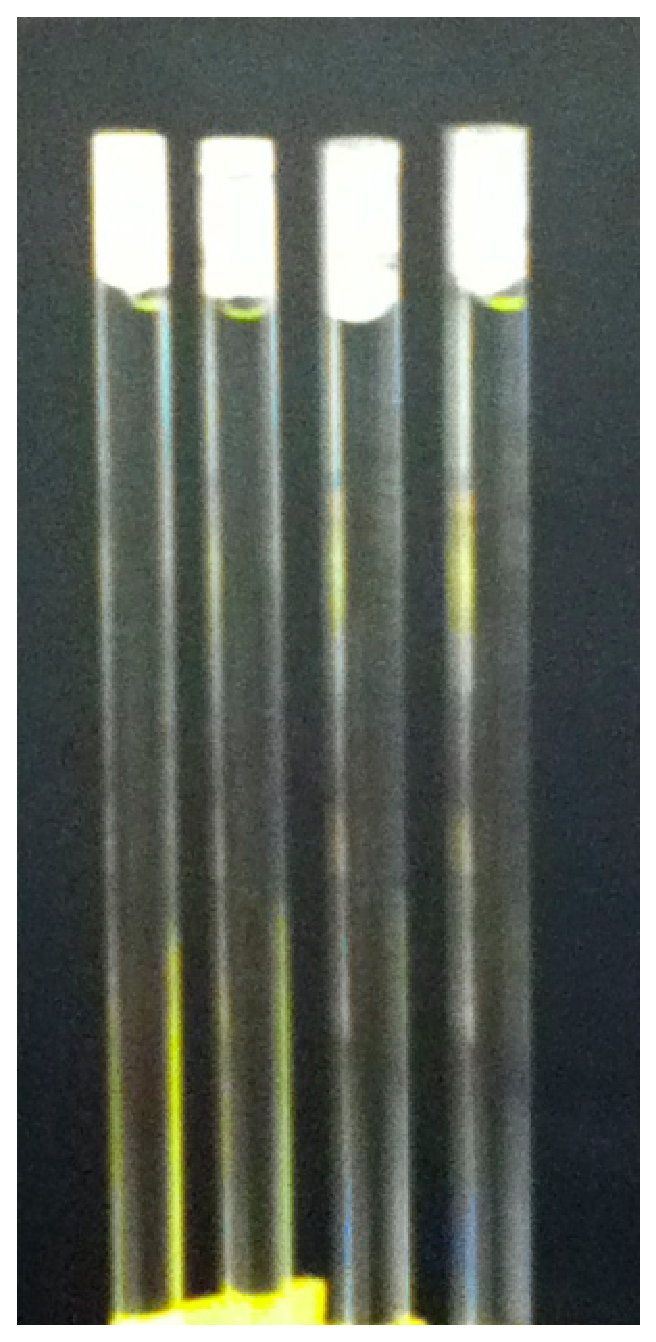
\includegraphics[width=1in]{phantom/images/tube_sealings/paraffin_and_floable_silicon.eps}}}
%     \centerline{\emph{(a) Paraffin wax at top with floatable silicon at bottom}}
%   \end{minipage}
%   \begin{minipage}[b]{1in}
%     \centering
%     \centerline{\mbox{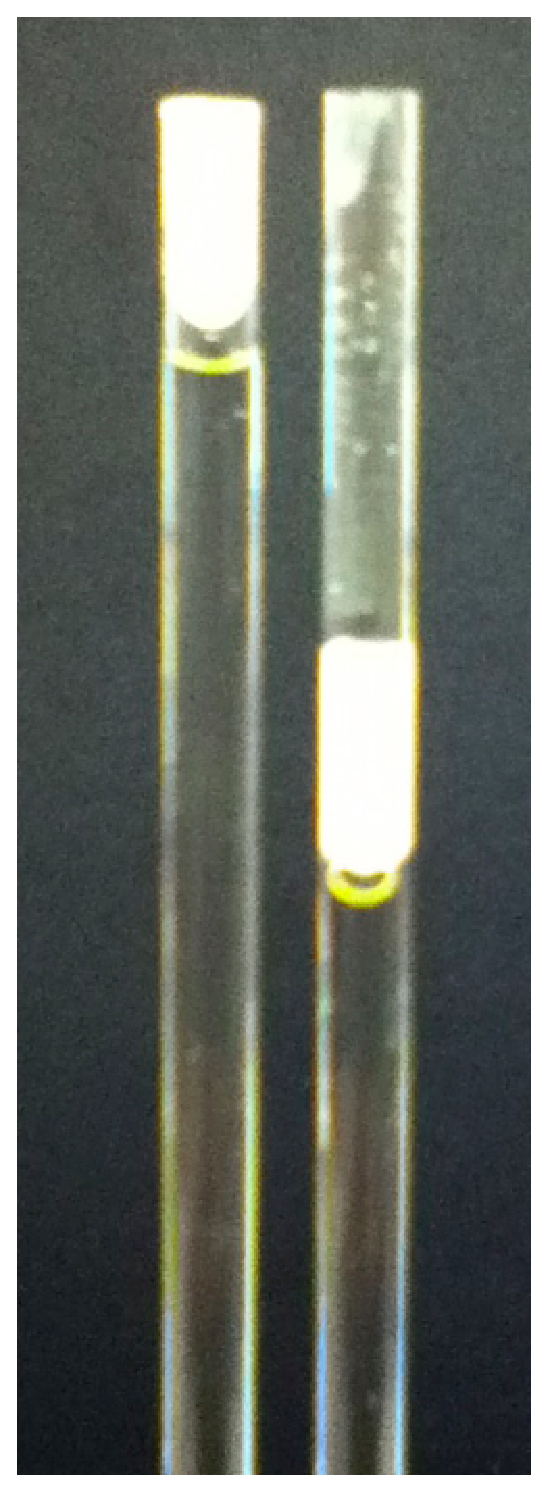
\includegraphics[width=1in]{phantom/images/tube_sealings/paraffin.eps}}}
%     \centerline{\emph{(b) Paraffin wax only}}
%   \end{minipage}

%   \begin{minipage}[b]{1in}
%     \centering
%     \centerline{\mbox{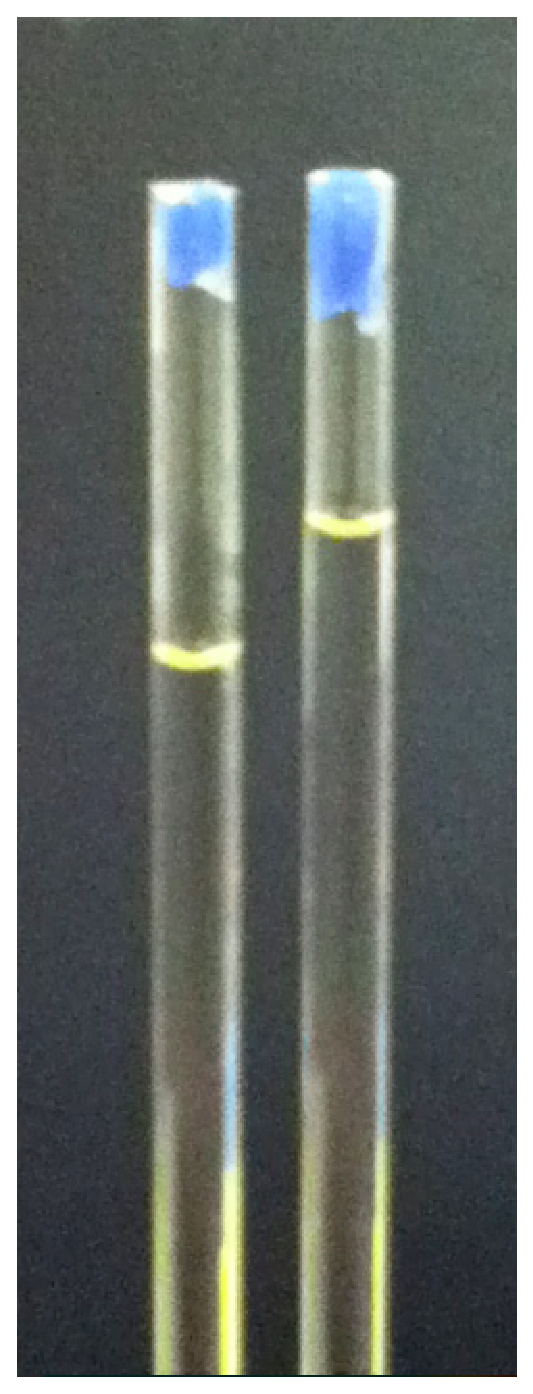
\includegraphics[width=1in]{phantom/images/tube_sealings/machinable_wax.eps}}}
%     \centerline{\emph{(c) Machinable wax}}
%   \end{minipage}\medskip
%   \begin{minipage}[b]{1in}
%     \centering
%     \centerline{\mbox{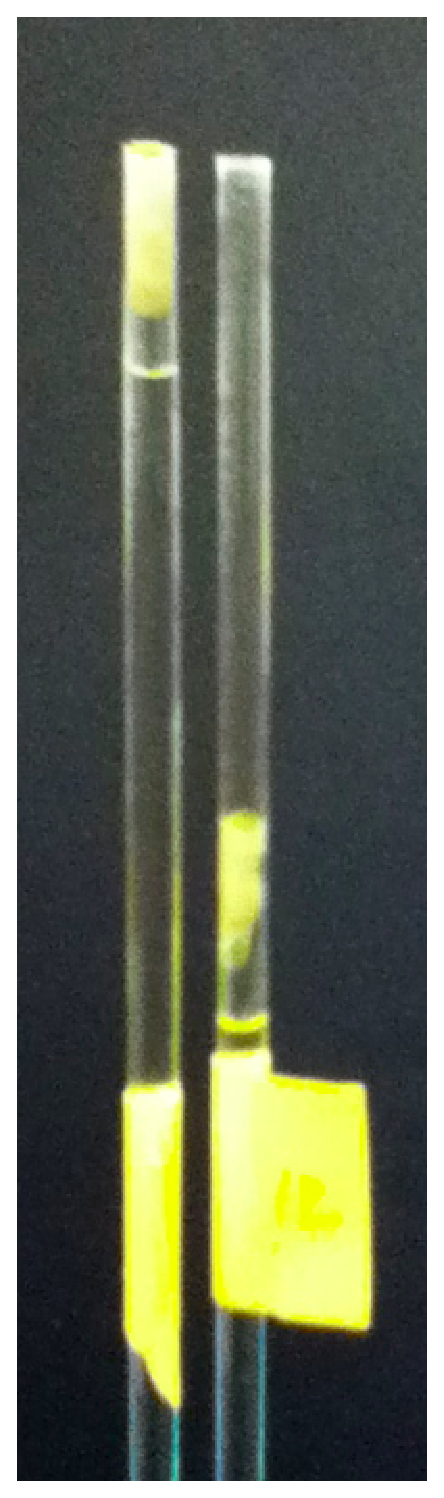
\includegraphics[width=1in]{phantom/images/tube_sealings/water_weld.eps}}}
%     \centerline{\emph{(d) Water weld}}
%   \end{minipage}

%   \begin{minipage}[b]{1in}
%     \centering
%     \centerline{\mbox{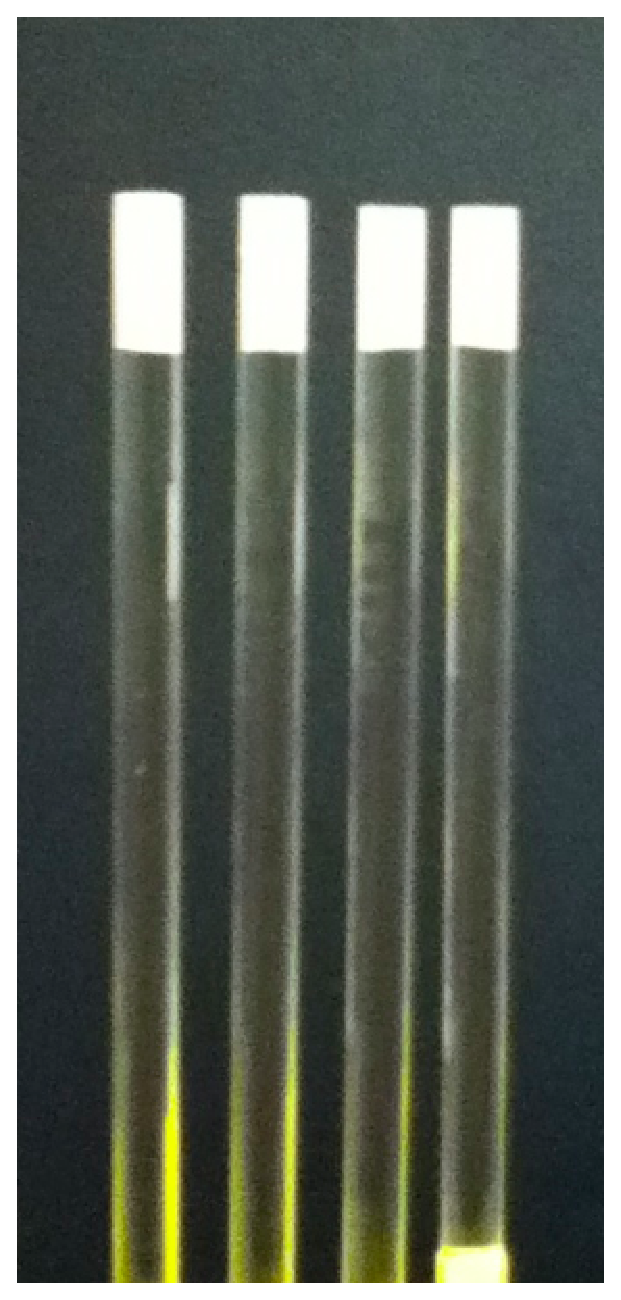
\includegraphics[width=1in]{phantom/images/tube_sealings/silicon.eps}}}
%     \centerline{\emph{(e) Silicon}}
%   \end{minipage}

% \end{figure}


\section{Installation and Use}

The new phantom is designed to rest in the head coil of a 3T MRI scanner.  It has a back plate with several
leveling screws to align the phantom in the head coil using the laser alignment system.  This alignment is
aided by alignment marks on the outside of the phantom. The phantom is then moved into the MRI scanner,
and its center is placed as close to the isocenter as possible.  While it is not required to be centered,
centering does improve the performance.  A quick alignment scan is used to ensure the phantom is in the best
location possible.  When this is done the scan is taken and processed using distortion detection and
correction software, which is not subject of the present presentation.

\section{Initial Experience}

The original phantom design, a 16-cm oil-filled cube, could not be scaled up due to weight and manufacturing
constraints. Our first modification was to look at changing the material to FR-4 since it is rigid, very flat,
and could be submerged for short periods of time to permit scanning the solid liquid interface in an MRI
machine.  Since most of the distortion is visible only in the corners, this was rapidly replaced by 8 corners
of a virtual cube, which could be connected by a rigid frame.  The weight of a tank to submerge either of
these designs to allow scanning was prohibitive, requiring a complete redesign.

\section{Conclusion}

A new phantom for the measurement and correction of nonlinear gradient field distortion of MRI systems is
presented.  It is lighter, more economic, and allows for both more accurate measurement of field distortion
and the location of the isocenter. 